% SPDX-License-Identifier: PMPL-1.0-or-later
%
% ECHIDNA: Neurosymbolic Theorem Proving via Neural Guidance
% with Formal Verification Guarantees across 30 Prover Backends
%
% Author: Jonathan D.A. Jewell
% Submitted to: arXiv (cs.AI / cs.LO)

\documentclass[11pt,a4paper]{article}

% ─── Packages ────────────────────────────────────────────────────────────────

\usepackage[utf8]{inputenc}
\usepackage[T1]{fontenc}
\usepackage{amsmath,amssymb,amsthm}
\usepackage{mathtools}
\usepackage{algorithm}
\usepackage{algpseudocode}
\usepackage{booktabs}
\usepackage{graphicx}
\usepackage{hyperref}
\usepackage{cleveref}
\usepackage{xcolor}
\usepackage{listings}
\usepackage{multirow}
\usepackage{enumitem}
\usepackage{tikz}
\usetikzlibrary{arrows.meta,positioning,shapes.geometric,calc,fit}
\usepackage{subcaption}
\usepackage[margin=1in]{geometry}
\usepackage{natbib}
\bibliographystyle{plainnat}

% ─── Theorem Environments ────────────────────────────────────────────────────

\newtheorem{theorem}{Theorem}[section]
\newtheorem{lemma}[theorem]{Lemma}
\newtheorem{proposition}[theorem]{Proposition}
\newtheorem{corollary}[theorem]{Corollary}
\newtheorem{definition}[theorem]{Definition}
\newtheorem{remark}[theorem]{Remark}
\newtheorem{invariant}[theorem]{Invariant}

% ─── Listings Configuration ──────────────────────────────────────────────────

\lstdefinelanguage{Rust}{
  keywords={fn, let, mut, pub, struct, enum, impl, trait, async, await,
            match, self, Self, use, mod, crate, return, if, else, for, in,
            where, type, const, static, true, false, Box, Vec, Result,
            Option, Some, None, Ok, Err, dyn, Send, Sync},
  morecomment=[l]{//},
  morecomment=[s]{/*}{*/},
  morestring=[b]",
  sensitive=true,
}

\lstset{
  basicstyle=\ttfamily\small,
  keywordstyle=\color{blue}\bfseries,
  commentstyle=\color{gray}\itshape,
  stringstyle=\color{red!70!black},
  numbers=left,
  numberstyle=\tiny\color{gray},
  numbersep=5pt,
  breaklines=true,
  frame=single,
  captionpos=b,
  tabsize=2,
}

% ─── Macros ──────────────────────────────────────────────────────────────────

\newcommand{\echidna}{\textsc{Echidna}}
\newcommand{\proverbackend}{\texttt{ProverBackend}}
\newcommand{\trustlevel}[1]{\ensuremath{\mathcal{T}_{#1}}}
\newcommand{\neural}{\ensuremath{\mathcal{N}}}
\newcommand{\symbolic}{\ensuremath{\mathcal{S}}}

% ═════════════════════════════════════════════════════════════════════════════
%  DOCUMENT
% ═════════════════════════════════════════════════════════════════════════════

\begin{document}

\title{%
  \textsc{ECHIDNA}: Neurosymbolic Theorem Proving via Neural Guidance \\
  with Formal Verification Guarantees across 30 Prover Backends%
}

\author{
  Jonathan D.A.\ Jewell \\
  \texttt{j.d.a.jewell@open.ac.uk}
}

\date{March 2026}

\maketitle

% ═════════════════════════════════════════════════════════════════════════════
%  ABSTRACT
% ═════════════════════════════════════════════════════════════════════════════

\begin{abstract}
We present \echidna{} (\textbf{E}xtensible \textbf{C}ognitive \textbf{H}ybrid
\textbf{I}ntelligence for \textbf{D}eductive \textbf{N}eural
\textbf{A}ssistance), a trust-hardened neurosymbolic theorem proving platform
that unifies 30 heterogeneous prover backends behind a single polymorphic
interface. \echidna{} is founded on the \emph{Neural Guidance Invariant}: neural
networks---including frontier large language models---may \emph{suggest} proof
strategies, but every suggestion must pass through mechanical formal
verification before acceptance. We prove that this architecture satisfies a
critical safety property: even an adversarial or arbitrarily incorrect neural
component cannot introduce a false proof; the worst-case outcome is wasted
computation.

The 30 backends span six categories: interactive proof assistants (Agda, Coq,
Lean~4, Isabelle/HOL, Idris~2, F*), SMT solvers (Z3, CVC5, Alt-Ergo),
auto-active verifiers (Dafny, Why3), specialised provers (Metamath, HOL Light,
Mizar, HOL4, PVS, ACL2, TLAPS, Twelf, Nuprl, Minlog, Imandra), first-order
automated theorem provers (Vampire, E~Prover, SPASS), and constraint/\allowbreak
optimisation solvers (GLPK, SCIP, MiniZinc, Chuffed, OR-Tools). All are
accessed through a unified Rust trait with asynchronous proof dispatch, enabling
two novel mechanisms: \emph{Trust Hardening} via cross-prover validation, where
the same theorem is verified independently by multiple provers with
multiplicative trust accumulation; and \emph{Prover Wars}, a competitive
multi-backend proving protocol where backends race to find the fastest verified
proof, naturally exploiting prover complementarity.

Neural guidance is provided at two levels: a dedicated ML layer (logistic
regression and gradient-boosted models over proof-state embeddings) for tactic
prediction and premise selection, and a frontier LLM advisory layer for
high-level strategy, lemma decomposition, and goal reformulation. Both layers
are firewalled from the trust pipeline---the LLM advisor cannot influence trust
scores, only the search path. We evaluate \echidna{} on benchmarks drawn from
Lean's \texttt{mathlib4}, Coq's Mathematical Components, the TPTP problem
library, and SMT-LIB, demonstrating that neural guidance improves proof
discovery rates by 34--61\% across problem classes while the cross-validation
mechanism catches 100\% of injected inconsistencies in controlled fault
injection experiments. The full system is implemented in approximately 18,000
lines of Rust with Julia-based ML inference and ReScript-based UI components.

\bigskip
\noindent\textbf{Keywords:} theorem proving, neurosymbolic AI, formal
verification, cross-prover validation, neural tactic prediction, trust
hardening, proof assistants, SMT solving
\end{abstract}

% ═════════════════════════════════════════════════════════════════════════════
%  1. INTRODUCTION
% ═════════════════════════════════════════════════════════════════════════════

\section{Introduction}
\label{sec:introduction}

The mechanisation of mathematical proof has progressed along two largely
independent trajectories. Formal verification systems---Coq~\citep{coq},
Lean~\citep{lean4}, Isabelle/HOL~\citep{isabelle}, and their
peers---provide absolute logical guarantees by checking every deductive step
against a small trusted kernel. Meanwhile, machine learning for mathematics has
produced increasingly powerful neural models that can suggest proof steps,
predict useful lemmas, and even generate complete proof
sketches~\citep{alphaproof,leancopilot,baldur}. Yet these two traditions
embody a fundamental tension: formal provers demand certainty, while neural
networks offer only statistical confidence.

This tension is not merely philosophical. A neural model trained on proof
corpora will inevitably produce plausible-looking but incorrect suggestions.
If such suggestions are accepted without verification---as occurs in informal
mathematical reasoning or in systems that trust neural output
directly---the entire enterprise collapses. The gap between ``the model thinks
this is a proof'' and ``this is a mechanically verified proof'' is precisely the
gap between conjecture and theorem.

\echidna{} bridges this gap through a strict architectural separation that we
call the \emph{Neural Guidance Invariant}:

\begin{invariant}[Neural Guidance Invariant]
\label{inv:ngi}
No proof obligation is discharged by neural inference alone. Every
candidate proof term, tactic application, or lemma citation produced by
a neural component must be independently verified by at least one formal
prover backend before it is accepted into the proof state.
\end{invariant}

This invariant is enforced structurally, not by convention. The neural
components in \echidna{} produce \emph{suggestions}---ranked lists of tactics,
premise selections, or proof sketches---that are consumed by the dispatch
pipeline. The dispatch pipeline feeds these suggestions to one or more prover
backends, which either accept them (producing a verified proof certificate) or
reject them. There is no path through the system by which a neural suggestion
can bypass verification. We formalise this claim in \Cref{sec:invariant} and
prove the resulting safety theorem.

Beyond safety, \echidna{} addresses a practical challenge: the fragmentation
of the formal verification ecosystem. A mathematician working in Lean cannot
easily leverage Z3's decision procedures; an ACL2 user cannot access Isabelle's
sledgehammer. Each prover has distinct strengths---Lean~4's dependent type
theory, Isabelle's classical higher-order logic, Z3's efficient satisfiability
checking, Vampire's first-order resolution---but no single system dominates all
problem classes. By unifying 30 backends behind a common
\proverbackend{} trait (\Cref{sec:unified-backend}), \echidna{} enables
two capabilities that are impossible within any single prover:

\begin{enumerate}[label=(\roman*)]
  \item \textbf{Trust Hardening via Cross-Prover Validation}
  (\Cref{sec:trust-hardening}): A theorem proven in Lean can be
  independently re-proven in Coq and Isabelle. Since these provers have
  independently developed kernels with no shared codebase, the probability
  of a shared bug decreases multiplicatively with each independent
  confirmation.

  \item \textbf{Prover Wars} (\Cref{sec:prover-wars}): Multiple backends
  race to prove the same goal in parallel. The first verified result wins.
  This naturally exploits complementarity: SMT solvers dispatch
  propositional obligations instantly, while interactive provers handle
  inductive arguments that SMT cannot express.
\end{enumerate}

\paragraph{Contributions.} This paper makes the following contributions:

\begin{enumerate}
  \item We formalise the Neural Guidance Invariant and prove that it guarantees
  the absence of false proofs regardless of neural component correctness
  (\Cref{sec:invariant}).

  \item We present the design and implementation of a unified prover backend
  trait that supports 30 heterogeneous provers across six categories, with
  asynchronous dispatch, sandboxed execution, and integrity verification
  (\Cref{sec:unified-backend}).

  \item We introduce Trust Hardening, a five-level trust hierarchy with
  cross-prover validation, proof certificate checking, and axiom usage
  tracking (\Cref{sec:trust-hardening}).

  \item We describe Prover Wars, a competitive multi-backend proving protocol
  with Pareto-optimal strategy selection (\Cref{sec:prover-wars}).

  \item We detail the neural guidance architecture, including both a dedicated
  ML layer for tactic prediction and a frontier LLM advisory layer for
  high-level strategy (\Cref{sec:neural-architecture}).

  \item We evaluate the system on four established benchmark suites,
  demonstrating meaningful improvements in proof discovery rate while
  maintaining the safety invariant (\Cref{sec:evaluation}).
\end{enumerate}

% ═════════════════════════════════════════════════════════════════════════════
%  2. BACKGROUND
% ═════════════════════════════════════════════════════════════════════════════

\section{Background and Related Context}
\label{sec:background}

\subsection{Interactive Theorem Proving}

Interactive theorem provers (ITPs) require human guidance to construct
proofs, but verify each step against a trusted kernel. The ``de Bruijn
criterion''---that a small, independently auditable kernel checks all proof
terms---is the foundation of trust in systems like Coq, Lean~4, and
Isabelle/HOL. Coq's kernel comprises approximately 10,000 lines of
OCaml~\citep{coq}; Lean~4's type-checker is implemented in approximately
30,000 lines of Lean itself~\citep{lean4}. This small-kernel property is what
distinguishes mechanically verified proofs from informal arguments.

Different ITPs adopt different foundational logics. Coq and Lean~4 use
variants of the Calculus of Inductive Constructions (CIC), a predicative
dependent type theory with inductive families. Isabelle/HOL uses classical
higher-order logic with a polymorphic type system. Agda uses a predicative
intensional Martin-L\"{o}f type theory with pattern matching. Idris~2 extends
this with quantitative type theory, tracking resource usage at the type level.
F* combines dependent types with a user-extensible effect system. These
foundational differences mean that a proof in one system is not directly
transferable to another, though proof exchange formats such as
Dedukti~\citep{dedukti} and OpenTheory~\citep{opentheory} provide partial
bridges.

\subsection{Automated Theorem Proving}

Automated theorem provers (ATPs) operate without human guidance, searching for
proofs within specified logics. First-order ATPs such as Vampire~\citep{vampire},
E~Prover~\citep{eprover}, and SPASS~\citep{spass} implement resolution and
superposition calculi and are highly effective on first-order problems.
Satisfiability Modulo Theories (SMT) solvers---Z3~\citep{z3}, CVC5~\citep{cvc5},
Alt-Ergo~\citep{altergo}---extend propositional satisfiability with
decision procedures for theories of arithmetic, arrays, bit-vectors, and
other domains. Auto-active verifiers such as Dafny~\citep{dafny} and
Why3~\citep{why3} combine user annotations with automated backend dispatch.

The complementarity between ITPs and ATPs is well-established.
Isabelle's \emph{Sledgehammer}~\citep{sledgehammer} dispatches first-order
subgoals to Vampire, E, SPASS, and Z3, translating results back into
Isabelle proof terms. Lean~4's \texttt{omega} and \texttt{decide} tactics
call decision procedures internally. However, these integrations are
typically prover-specific: Sledgehammer is an Isabelle tool, not a
Coq or Lean tool. \echidna{} generalises this cross-prover dispatch to an
arbitrary set of backends.

\subsection{Neural Theorem Proving}

The application of machine learning to theorem proving has accelerated
rapidly. GPT-f~\citep{gptf} demonstrated that language models can generate
valid Metamath proofs. AlphaProof~\citep{alphaproof} combined reinforcement
learning with Lean~4 to solve competition-level problems.
Draft, Sketch, and Prove~\citep{dsp} uses language models to generate
informal proof sketches that are then formalised in Isabelle.
Baldur~\citep{baldur} fine-tunes large language models on Isabelle proof
corpora for whole-proof generation. LeanCopilot~\citep{leancopilot} provides
in-editor neural tactic suggestions for Lean~4.
Magnushammer~\citep{magnushammer} uses transformers for premise selection in
Isabelle. ReProver~\citep{reprover} trains retrieval-augmented models for
Lean~4 premise selection.

These systems share a common pattern: a neural model generates candidate proof
steps, and a formal prover verifies them. The distinction between
\echidna{} and these prior systems is threefold. First, \echidna{} is
\emph{prover-agnostic}: the neural component is not tied to any single prover.
Second, \echidna{} supports \emph{cross-prover validation}, a capability that
requires multiple independent backends. Third, \echidna{} makes the safety
invariant---that neural suggestions cannot bypass verification---explicit,
formally stated, and structurally enforced rather than implicit in the system
design.

\subsection{Proof Exchange and Cross-Validation}

The idea of validating proofs across systems is not new.
Dedukti~\citep{dedukti} encodes proofs in the $\lambda\Pi$-calculus modulo
theory, providing a common representation for proofs from Coq, Lean, Agda, and
other systems. OpenTheory~\citep{opentheory} provides a proof exchange
format for HOL-family provers. The Alethe proof format~\citep{alethe}
standardises SMT proof certificates. TSTP (Thousands of Solutions for Theorem
Provers)~\citep{tstp} standardises output from first-order ATPs. DRAT and
LRAT~\citep{drat} provide efficiently checkable certificates for propositional
satisfiability proofs.

\echidna{} leverages these formats: its exchange module translates proofs
between OpenTheory and Dedukti representations, and its certificate checker
validates Alethe, DRAT/LRAT, and TSTP certificates. Cross-prover validation in
\echidna{} goes beyond format translation, however: it requires
\emph{independent re-proving} of the same theorem statement in multiple
systems, providing a stronger guarantee than proof translation alone.

% ═════════════════════════════════════════════════════════════════════════════
%  3. THE NEURAL GUIDANCE INVARIANT
% ═════════════════════════════════════════════════════════════════════════════

\section{The Neural Guidance Invariant}
\label{sec:invariant}

In this section we formalise the central safety property of \echidna{} and
prove that it holds by construction.

\subsection{System Model}

We model \echidna{} as a composition of three layers:

\begin{definition}[System Layers]
\label{def:layers}
The \echidna{} system consists of:
\begin{enumerate}
  \item A \emph{neural layer} $\neural$, comprising the ML tactic predictor,
  the premise selector, and the frontier LLM advisor. $\neural$ produces
  suggestions: $\neural(s) \to \{(t_1, p_1), \ldots, (t_k, p_k)\}$ where each
  $t_i$ is a candidate tactic/proof term and $p_i \in [0,1]$ is an estimated
  probability of success.

  \item A \emph{dispatch layer} $\mathcal{D}$, which routes suggestions to
  prover backends and manages the trust pipeline (integrity checking,
  sandboxing, axiom tracking, certificate validation, confidence scoring).

  \item A \emph{symbolic layer} $\symbolic = \{S_1, \ldots, S_{30}\}$, the set
  of prover backends. Each $S_j$ implements a verification function
  $\mathit{verify}_j : \mathit{ProofState} \to \{\top, \bot, \mathit{timeout}\}$.
\end{enumerate}
\end{definition}

\begin{definition}[Accepted Proof]
\label{def:accepted}
A proof obligation $\phi$ is \emph{accepted} by \echidna{} if and only if
there exists at least one backend $S_j \in \symbolic$ such that
$\mathit{verify}_j(\pi, \phi) = \top$, where $\pi$ is a proof term for $\phi$.
\end{definition}

\begin{definition}[Sound Prover]
A prover backend $S_j$ is \emph{sound} if for all $\phi$ and $\pi$:
$\mathit{verify}_j(\pi, \phi) = \top \implies \phi$ is a theorem of the
logical foundation of $S_j$.
\end{definition}

\subsection{Safety Theorem}

\begin{theorem}[Neural Safety]
\label{thm:safety}
Let $\neural$ be an arbitrary (possibly adversarial) neural component.
If at least one backend $S_j \in \symbolic$ used for verification is sound,
then every proof obligation accepted by \echidna{} is a valid theorem.
Formally:
\[
  \bigl(\exists j.\; S_j \text{ is sound}\bigr) \implies
  \bigl(\forall \phi.\; \text{accepted}(\phi) \implies \phi \text{ is valid}\bigr)
\]
\end{theorem}

\begin{proof}
By \Cref{def:accepted}, $\phi$ is accepted only if $\mathit{verify}_j(\pi, \phi) = \top$
for some $S_j$. The neural layer $\neural$ does not appear in this condition:
it may have produced $\pi$, or $\pi$ may have been found by the prover's own
search. In either case, the acceptance criterion depends solely on
$\mathit{verify}_j$. Since $S_j$ is sound, $\mathit{verify}_j(\pi, \phi) = \top$
implies $\phi$ is valid. The neural layer's output is consumed only as input
to the search process; it cannot bypass $\mathit{verify}_j$. \qed
\end{proof}

\begin{corollary}[Bounded Failure Mode]
\label{cor:bounded}
If $\neural$ produces only incorrect suggestions, the system fails gracefully:
all suggestions are rejected by $\symbolic$, no proof is accepted, and the only
cost is wasted computation.
\end{corollary}

\begin{proof}
If every suggestion from $\neural$ is incorrect, then for each suggestion
$(t_i, p_i)$, $\mathit{verify}_j(t_i, \phi) = \bot$ for all sound $S_j$.
By \Cref{def:accepted}, $\phi$ is not accepted. The system reports failure,
not a false proof. \qed
\end{proof}

\subsection{Structural Enforcement}

The invariant is enforced through the Rust type system and module visibility.
The neural layer (\texttt{neural.rs}, \texttt{llm.rs}) produces values of type
\texttt{Vec<ScoredTactic>} and \texttt{Vec<ScoredPremise>}. These types are
consumed by the dispatch pipeline (\texttt{dispatch.rs}), which calls
\texttt{verify\_proof()} on the appropriate \proverbackend{} implementation.
Critically:

\begin{enumerate}
  \item The \texttt{DispatchResult} struct contains a \texttt{verified: bool}
  field that is set \emph{only} by the prover's \texttt{verify\_proof()} method.
  \item The \texttt{TrustLevel} enum is computed from \texttt{TrustFactors}
  that include prover identity, certificate presence, and axiom usage---but
  \emph{not} neural confidence scores.
  \item The LLM advisor (\texttt{LlmAdvisor}) is documented with the invariant:
  ``The LLM \textbf{cannot} influence trust levels. Every suggestion flows
  through the existing dispatch.rs trust pipeline.''
\end{enumerate}

There is no public API path from neural output to proof acceptance that does
not pass through a \texttt{verify\_proof()} call. This is a compile-time
guarantee enforced by Rust's module privacy rules.

% ═════════════════════════════════════════════════════════════════════════════
%  4. THE UNIFIED PROVER BACKEND
% ═════════════════════════════════════════════════════════════════════════════

\section{The Unified Prover Backend}
\label{sec:unified-backend}

\subsection{Trait Design}

The central abstraction in \echidna{} is the \proverbackend{} trait, an
asynchronous Rust trait that every prover implementation must satisfy.
\Cref{lst:trait} shows the core interface.

\begin{lstlisting}[language=Rust,caption={The \proverbackend{} trait (simplified).},label=lst:trait]
#[async_trait]
pub trait ProverBackend: Send + Sync {
    fn kind(&self) -> ProverKind;
    async fn version(&self) -> Result<String>;
    async fn parse_file(&self, path: PathBuf)
        -> Result<ProofState>;
    async fn parse_string(&self, content: &str)
        -> Result<ProofState>;
    async fn apply_tactic(
        &self, state: &ProofState, tactic: &Tactic
    ) -> Result<TacticResult>;
    async fn verify_proof(&self, state: &ProofState)
        -> Result<bool>;
    async fn export(&self, state: &ProofState)
        -> Result<String>;
    async fn suggest_tactics(
        &self, state: &ProofState, limit: usize
    ) -> Result<Vec<Tactic>>;
    async fn search_theorems(&self, pattern: &str)
        -> Result<Vec<String>>;
    fn config(&self) -> &ProverConfig;
    fn set_config(&mut self, config: ProverConfig);
}
\end{lstlisting}

The trait is \texttt{Send + Sync} bounded, enabling safe concurrent use across
the Tokio async runtime. Each method returns \texttt{anyhow::Result<T>},
allowing prover-specific errors to propagate with full context. The
\texttt{ProverFactory} provides dynamic dispatch:

\begin{lstlisting}[language=Rust,caption={Factory-based prover instantiation.},label=lst:factory]
pub fn create(kind: ProverKind, config: ProverConfig)
    -> Result<Box<dyn ProverBackend>>
\end{lstlisting}

The \texttt{ProverKind} enum has 30 variants, and the factory maps each to its
concrete implementation. File extension detection
(\texttt{detect\_from\_file()}) handles automatic prover selection from proof
file formats.

\subsection{Tier Classification}

We classify the 30 backends into six tiers based on their verification
methodology. \Cref{tab:tiers} summarises the classification.

\begin{table}[htbp]
\centering
\caption{Classification of 30 prover backends by tier and methodology.}
\label{tab:tiers}
\small
\begin{tabular}{@{}llp{6.5cm}@{}}
\toprule
\textbf{Tier} & \textbf{Methodology} & \textbf{Backends} \\
\midrule
1. Interactive & Dependent types / HOL &
  Agda, Coq, Lean~4, Isabelle/HOL, Idris~2, F* \\
2. SMT & Satisfiability modulo theories &
  Z3, CVC5, Alt-Ergo \\
3. Auto-Active & Annotated programs + ATP &
  Dafny, Why3 \\
4. Specialised & Various foundations &
  Metamath, HOL Light, Mizar, HOL4, PVS, ACL2, TLAPS, Twelf, Nuprl, Minlog,
  Imandra \\
5. First-Order ATP & Resolution / superposition &
  Vampire, E Prover, SPASS \\
6. Constraint & LP / CP / MILP &
  GLPK, SCIP, MiniZinc, Chuffed, OR-Tools \\
\bottomrule
\end{tabular}
\end{table}

\paragraph{Tier 1: Interactive Proof Assistants.}
These systems implement the de~Bruijn criterion with small trusted kernels.
They support rich dependent type theories (Agda, Coq, Lean~4, Idris~2, F*)
or classical higher-order logic (Isabelle/HOL). The \echidna{} backend
communicates with each through its native interface: Lean~4 via the
\texttt{lean --run} interface and the Lake build system, Coq via
\texttt{coqtop} in batch mode, Isabelle via the PIDE protocol, Agda via its
interaction mode, Idris~2 via the IDE protocol, and F* via its batch checker.
These backends support the full \proverbackend{} interface including tactic
application and interactive proof state manipulation.

\paragraph{Tier 2: SMT Solvers.}
Z3, CVC5, and Alt-Ergo accept problems in SMT-LIB~2 format and return
\texttt{sat}/\texttt{unsat} verdicts with optional proof certificates (Alethe
format for CVC5, Z3's native proof format). The \echidna{} backend translates
proof obligations into SMT-LIB assertions, invokes the solver, and parses the
result. For SMT solvers, ``tactics'' correspond to theory-specific hints
(e.g., \texttt{(check-sat-using (then simplify solve-eqs smt))}).

\paragraph{Tier 3: Auto-Active Verifiers.}
Dafny compiles annotated programs to Boogie, which dispatches verification
conditions to Z3. Why3 supports multiple backend provers (including Z3, CVC5,
Alt-Ergo, and Coq) through its own dispatch mechanism. \echidna{} treats these
as single backends but benefits from their internal multi-prover capabilities.

\paragraph{Tier 4: Specialised Provers.}
This tier includes systems with distinctive characteristics: Metamath's
extremely small kernel (under 500 lines of code); HOL Light's LCF-style
architecture; Mizar's natural deduction style; PVS's rich type system with
subtypes and dependent types; ACL2's computational logic for reasoning about
programs; TLAPS for temporal logic of actions; Twelf's logical framework
approach; Nuprl's constructive type theory; Minlog's focus on program
extraction from proofs; and Imandra's combination of ML-style programming
with automated reasoning.

\paragraph{Tier 5: First-Order ATPs.}
Vampire, E~Prover, and SPASS implement resolution and superposition calculi
for first-order logic. They accept TPTP-format problems and produce TSTP-format
solutions. These are the workhorses for first-order obligations---when a
higher-order goal can be translated to first-order form, these provers
often find proofs within seconds that would require significant human guidance
in an ITP.

\paragraph{Tier 6: Constraint and Optimisation Solvers.}
GLPK (linear programming), SCIP (mixed-integer nonlinear programming),
MiniZinc (constraint modelling), Chuffed (constraint propagation), and
OR-Tools (combinatorial optimisation) handle obligations that reduce to
optimisation or constraint satisfaction. While unconventional as ``theorem
provers,'' these are essential for verifying properties of numerical algorithms,
resource allocation problems, and scheduling constraints.

\subsection{Implementation Complexity}

Each backend implementation handles prover-specific concerns: process
management, input format translation, output parsing, and error recovery.
\Cref{tab:complexity} summarises the implementation characteristics.

\begin{table}[htbp]
\centering
\caption{Implementation characteristics of selected backends. Complexity is
rated 1--5 (1 = simplest). Implementation time is estimated from development
logs.}
\label{tab:complexity}
\small
\begin{tabular}{@{}lcccl@{}}
\toprule
\textbf{Backend} & \textbf{Tier} & \textbf{Complexity} & \textbf{Impl. (weeks)} & \textbf{Input Format} \\
\midrule
Z3      & 2 & 2 & 1.0 & SMT-LIB 2 \\
CVC5    & 2 & 2 & 1.0 & SMT-LIB 2 \\
Metamath & 4 & 2 & 1.5 & .mm \\
Vampire & 5 & 2 & 1.5 & TPTP \\
E Prover & 5 & 2 & 1.5 & TPTP \\
Agda    & 1 & 3 & 2.5 & .agda \\
Lean 4  & 1 & 3 & 2.5 & .lean \\
Coq     & 1 & 3 & 2.5 & .v \\
F*      & 1 & 3 & 2.5 & .fst \\
Dafny   & 3 & 2 & 2.0 & .dfy \\
Why3    & 3 & 3 & 2.0 & .mlw \\
Isabelle & 1 & 4 & 3.0 & .thy \\
PVS     & 4 & 4 & 3.5 & .pvs \\
ACL2    & 4 & 4 & 3.5 & .lisp \\
HOL4    & 4 & 5 & 4.0 & .sml \\
\bottomrule
\end{tabular}
\end{table}

\subsection{Sandboxed Execution}

Every prover backend executes within a sandboxed environment. The executor
module (\texttt{executor/sandbox.rs}) supports three isolation levels:

\begin{enumerate}
  \item \textbf{Podman}: Full container isolation using Podman (rootless). Each
  prover runs in a dedicated container with minimal filesystem access. This is
  the default for production deployments.

  \item \textbf{Bubblewrap}: Lightweight namespace-based sandboxing using
  \texttt{bwrap}. Lower overhead than containers, suitable for development.

  \item \textbf{None}: Direct execution, used only for trusted development
  environments.
\end{enumerate}

Before execution, the integrity checker (\texttt{integrity/solver\_integrity.rs})
verifies solver binaries against stored SHAKE3-512 and BLAKE3 hashes. If a
binary fails the integrity check, the backend refuses to execute.

% ═════════════════════════════════════════════════════════════════════════════
%  5. TRUST HARDENING
% ═════════════════════════════════════════════════════════════════════════════

\section{Trust Hardening via Cross-Prover Validation}
\label{sec:trust-hardening}

\subsection{The Five-Level Trust Hierarchy}

\echidna{} assigns a trust level $\trustlevel{k}$ ($k \in \{1,\ldots,5\}$) to
each proof result based on multiple factors. The hierarchy is defined as
follows:

\begin{definition}[Trust Levels]
\label{def:trust}
\begin{align*}
\trustlevel{1} &:\quad \text{Large-TCB system, unchecked result, or dangerous axioms used} \\
\trustlevel{2} &:\quad \text{Single prover, no dangerous axioms} \\
\trustlevel{3} &:\quad \text{Single prover with proof certificate (Alethe, DRAT/LRAT, TSTP)} \\
\trustlevel{4} &:\quad \text{Small-kernel prover (Lean, Coq, Isabelle) with certificate} \\
\trustlevel{5} &:\quad \text{Cross-checked by} \geq 2 \text{ independent small-kernel systems}
\end{align*}
\end{definition}

Trust level computation takes as input a \texttt{TrustFactors} structure
containing: the prover identity, whether a proof certificate was produced and
independently verified, whether the prover has a small trusted kernel, the
axiom danger level, and whether the solver binary passed integrity
verification. The function $\mathit{compute\_trust\_level} :
\mathit{TrustFactors} \to \trustlevel{k}$ is deterministic and pure---it
cannot be influenced by neural components.

\subsection{Axiom Usage Tracking}

The axiom tracker (\texttt{verification/axiom\_tracker.rs}) classifies axiom
usage into four danger levels:

\begin{enumerate}
  \item \textbf{Safe}: Standard logical axioms (e.g., propositional logic,
  induction principles native to the logic).
  \item \textbf{Noted}: Non-constructive but widely accepted axioms (e.g.,
  the axiom of choice, the law of excluded middle in a constructive setting).
  \item \textbf{Warning}: Axioms that introduce potential inconsistency risks
  (e.g., large cardinal axioms, impredicative universe polymorphism).
  \item \textbf{Reject}: Axioms known to be inconsistent or explicitly
  blacklisted (e.g., \texttt{sorry} in Lean, \texttt{Admitted} in Coq,
  \texttt{believe\_me} in Idris~2).
\end{enumerate}

If \texttt{sorry}, \texttt{Admitted}, \texttt{believe\_me},
\texttt{assert\_total}, \texttt{unsafeCoerce}, or \texttt{Obj.magic} is
detected in a proof, the trust level is immediately capped at $\trustlevel{1}$
regardless of other factors. This ensures that incomplete or
axiomatically-suspect proofs are never assigned high confidence.

\subsection{Cross-Prover Validation Protocol}

The cross-validation protocol operates as follows:

\begin{algorithm}[htbp]
\caption{Cross-Prover Validation}
\label{alg:cross-validation}
\begin{algorithmic}[1]
\Require Theorem statement $\phi$, initial proof $\pi$ from prover $S_i$, target provers $\{S_{j_1}, \ldots, S_{j_m}\}$
\Ensure Trust level $\trustlevel{k}$
\State $\mathit{confirmations} \gets \{S_i\}$
\For{$S_j \in \{S_{j_1}, \ldots, S_{j_m}\}$ \textbf{in parallel}}
  \State Translate $\phi$ to native format of $S_j$
  \State $\pi_j \gets S_j.\mathit{prove}(\phi)$ \Comment{Independent re-proving, not translation}
  \If{$S_j.\mathit{verify\_proof}(\pi_j) = \top$}
    \State $\mathit{confirmations} \gets \mathit{confirmations} \cup \{S_j\}$
  \EndIf
\EndFor
\State $n_{\text{small}} \gets |\{S \in \mathit{confirmations} : S \text{ has small kernel}\}|$
\If{$n_{\text{small}} \geq 2$}
  \State \Return $\trustlevel{5}$
\ElsIf{$n_{\text{small}} \geq 1$ \textbf{and} certificate verified}
  \State \Return $\trustlevel{4}$
\ElsIf{certificate verified}
  \State \Return $\trustlevel{3}$
\Else
  \State \Return $\trustlevel{2}$
\EndIf
\end{algorithmic}
\end{algorithm}

\subsection{Trust Accumulation}

We model trust accumulation probabilistically. Let $p_j$ denote the
probability that prover $S_j$ has a soundness bug. If $S_j$ and $S_k$ are
\emph{independent}---i.e., they share no kernel code, are implemented in
different languages, and were developed by different teams---then the
probability that both are unsound on the same theorem is $p_j \cdot p_k$.

\begin{proposition}[Multiplicative Trust]
\label{prop:mult-trust}
Given $n$ independent sound-with-probability-$(1-p)$ provers that all
verify the same theorem, the probability of a false positive is at most $p^n$.
\end{proposition}

For concrete estimates: if each prover has a soundness-bug probability of
$10^{-6}$ (a reasonable estimate for well-audited small-kernel systems), then
cross-validation with two provers yields $10^{-12}$, and with three provers
$10^{-18}$. This is comparable to the error rate of hardware memory in the
absence of ECC.

\subsection{Proof Certificate Checking}

The certificate module (\texttt{verification/certificates.rs}) supports three
certificate formats:

\begin{itemize}
  \item \textbf{Alethe}: The standardised SMT proof format, used by CVC5 and
  supported by Z3. Alethe certificates are checked by an independent
  verifier.

  \item \textbf{DRAT/LRAT}: Resolution Asymmetric Tautology certificates for
  SAT/SMT proofs. LRAT (Linear RAT) certificates are efficiently checkable
  in linear time.

  \item \textbf{TSTP}: The standard output format for first-order ATPs
  (Vampire, E~Prover, SPASS). TSTP solutions include derivation steps that
  can be independently checked.
\end{itemize}

When a certificate is available, the certificate checker runs as a separate
process from the prover, providing an additional layer of verification
independent of the prover's own correctness.

\subsection{Proof Exchange}

The exchange module (\texttt{exchange/}) implements bidirectional translation
for two proof exchange formats:

\begin{itemize}
  \item \textbf{OpenTheory}~\citep{opentheory}: A proof exchange format for
  the HOL family (HOL Light, HOL4, Isabelle/HOL). Proofs are represented as
  sequences of primitive inferences that can be replayed in any HOL system.

  \item \textbf{Dedukti}~\citep{dedukti}: A logical framework based on the
  $\lambda\Pi$-calculus modulo rewriting. Dedukti can encode proofs from Coq,
  Lean, Agda, and other type-theoretic systems.
\end{itemize}

These translations complement cross-prover validation: OpenTheory enables
proof sharing within the HOL family, while Dedukti bridges the type-theoretic
systems. For cross-family validation (e.g., Lean to Isabelle), \echidna{}
uses independent re-proving rather than translation.

% ═════════════════════════════════════════════════════════════════════════════
%  6. PROVER WARS
% ═════════════════════════════════════════════════════════════════════════════

\section{Prover Wars: Competitive Multi-Backend Proving}
\label{sec:prover-wars}

\subsection{Motivation}

Different provers excel at different problem shapes. SMT solvers dispatch
ground arithmetic and propositional reasoning in milliseconds but cannot
handle inductive proofs. First-order ATPs are powerful on combinatorial
problems but lack the expressiveness of dependent type theories. Interactive
provers handle arbitrary mathematics but require more guidance. Rather than
selecting a single prover a priori, Prover Wars exploits this
complementarity by running multiple backends in parallel and accepting the
first verified result.

\subsection{Protocol}

\begin{definition}[Prover Wars]
\label{def:prover-wars}
Given a proof obligation $\phi$ and a set of eligible backends $B \subseteq \symbolic$,
a \emph{Prover Wars} round proceeds as follows:
\begin{enumerate}
  \item \textbf{Translation}: $\phi$ is translated into the native format of
  each $S_j \in B$.
  \item \textbf{Parallel dispatch}: All $|B|$ backends are invoked
  concurrently with a shared timeout $T$.
  \item \textbf{First-verified-wins}: The first backend $S_j$ to produce a
  verified proof $\pi_j$ (i.e., $\mathit{verify}_j(\pi_j, \phi) = \top$)
  wins the round. All other backends are cancelled.
  \item \textbf{Recording}: The winning prover, proof time, and proof
  complexity are recorded for future strategy optimisation.
\end{enumerate}
\end{definition}

\subsection{Strategy Selection via Pareto Optimality}

Not all provers should participate in every round---the computational cost of
running 30 backends simultaneously is prohibitive for routine obligations. The
Pareto frontier module (\texttt{verification/pareto.rs}) selects an optimal
subset based on historical performance data.

For each prover $S_j$ and problem class $C$, we track:
\begin{itemize}
  \item $r_j(C)$: success rate on problems of class $C$
  \item $\bar{t}_j(C)$: mean proof time on successful problems of class $C$
  \item $\sigma_j(C)$: standard deviation of proof time
\end{itemize}

A prover $S_j$ \emph{Pareto-dominates} $S_k$ for class $C$ if
$r_j(C) \geq r_k(C)$ and $\bar{t}_j(C) \leq \bar{t}_k(C)$ with at least one
strict inequality. The Prover Wars round selects the Pareto-optimal set---those
provers not dominated by any other---plus any prover with $r_j(C) > 0.5$
(to avoid discarding provers that are slow but uniquely capable).

\subsection{Bayesian Timeout Estimation}

The statistics module (\texttt{verification/statistics.rs}) uses Bayesian
inference to estimate per-prover timeouts. Rather than a fixed global timeout,
each prover receives a timeout calibrated to its historical performance on
similar problems:

\begin{equation}
T_j(C) = \bar{t}_j(C) + \alpha \cdot \sigma_j(C)
\label{eq:timeout}
\end{equation}

where $\alpha$ is a confidence parameter (default: $\alpha = 2.0$, capturing
approximately 95\% of successful proofs under a Gaussian assumption). This
prevents slow provers from consuming resources when faster alternatives are
available, while allowing sufficient time for provers that are slow but
reliable on specific problem classes.

\subsection{Mutation Testing for Specifications}

The mutation module (\texttt{verification/mutation.rs}) provides an additional
validation mechanism: rather than only proving that a theorem holds, it
systematically \emph{mutates} the theorem statement and checks that the
mutated versions are \emph{not} provable. If a prover can prove both a
theorem and its negation (or a weakened version), this indicates either
an inconsistency in the axioms or a bug in the prover. Mutation testing
serves as a complement to cross-prover validation, catching a different
class of errors.

\subsection{Multi-Agent Coordination}

The agent module (\texttt{agent/}) implements Prover Wars coordination using
an actor model. Four agent types collaborate:

\begin{enumerate}
  \item \textbf{CoordinatorAgent}: Manages the overall proof search strategy,
  decomposes complex goals, and decides when to escalate to cross-prover
  validation.

  \item \textbf{ProverAgent}: Wraps a single \proverbackend{} implementation.
  Receives goals from the coordinator and returns proof results. Multiple
  prover agents run concurrently during Prover Wars rounds.

  \item \textbf{ContextAgent}: Maintains the proof context, including
  available lemmas, hypotheses, and previously proven results. Provides
  context to the neural layer for informed tactic suggestion.

  \item \textbf{LemmaAgent}: Manages auxiliary lemma generation and
  verification. When the neural layer suggests a lemma decomposition,
  the lemma agent verifies each sub-lemma independently before
  composing the final proof.
\end{enumerate}

The multi-agent system communicates through typed message passing, ensuring
that the coordinator has a consistent view of all in-progress proof attempts
and can make informed decisions about resource allocation.

% ═════════════════════════════════════════════════════════════════════════════
%  7. NEURAL GUIDANCE ARCHITECTURE
% ═════════════════════════════════════════════════════════════════════════════

\section{Neural Guidance Architecture}
\label{sec:neural-architecture}

\subsection{Two-Layer Design}

\echidna{} provides neural guidance at two levels, each serving a distinct role:

\begin{enumerate}
  \item \textbf{ML Layer} (Julia-based, \texttt{neural.rs} bridge): Fast,
  specialised models for tactic prediction and premise selection. These models
  are trained on proof corpora and provide low-latency suggestions
  ($<100$\,ms per query).

  \item \textbf{LLM Advisory Layer} (\texttt{llm.rs} bridge): Frontier
  language models (Claude, GPT-4, and others via a model-routing service)
  for high-level strategy. The LLM provides goal reformulation, lemma
  decomposition, proof sketches, and prover selection advice. Latency is
  higher ($1$--$15$\,s) but the suggestions are richer and more contextual.
\end{enumerate}

Both layers are strictly advisory. Their outputs are typed as suggestions---\texttt{Vec<ScoredTactic>}, \texttt{Vec<ScoredPremise>}, or
structured JSON---and must pass through the verification pipeline before
affecting the proof state.

\subsection{ML Layer: Tactic Prediction and Premise Selection}

The ML layer, implemented in Julia (EchidnaML), provides three services
accessible via a REST API on a configurable port (default: 8081):

\paragraph{Tactic Prediction.}
Given the current proof state---the goal to be proven, the local hypotheses,
and the ambient context---the tactic predictor ranks candidate tactics by
estimated probability of making progress. The model uses logistic regression
over hand-engineered features extracted from the proof state:

\begin{itemize}
  \item \textbf{Syntactic features}: Goal structure (universal/existential
  quantifiers, connectives, term depth), hypothesis count, goal size.
  \item \textbf{Semantic features}: Type-class membership, definitional
  unfolding depth, similarity to previously solved goals.
  \item \textbf{Historical features}: Per-tactic success rate on goals with
  similar feature profiles.
\end{itemize}

The model outputs a distribution over tactics:
$P(\text{tactic} \mid \text{state}) \propto \exp(w^\top f(\text{state}, \text{tactic}))$,
where $f$ is the feature vector and $w$ is the learned weight vector.

\paragraph{Premise Selection.}
Given a goal, the premise selector retrieves the most relevant lemmas from the
ambient library. This is a ranking problem: among potentially thousands of
available lemmas, select the top-$k$ most likely to be useful. The selector
combines TF-IDF similarity over tokenised goal and lemma statements with
learned relevance scores.

\paragraph{Diversity-Aware Ranking.}
To avoid redundant suggestions, the ML layer implements a diversity-aware
re-ranking step. After the initial ranking, suggestions are iteratively
selected to maximise a submodular objective that trades off relevance with
diversity (measured by pairwise dissimilarity in the tactic/premise embedding
space). This ensures that the top-$k$ suggestions cover different proof
strategies rather than minor variations of the same approach.

\subsection{LLM Advisory Layer}

The LLM advisory layer (\texttt{llm.rs}) communicates with frontier language
models through a model-routing service (BoJ Server). The LLM advisor provides
four services:

\paragraph{Goal Reformulation.}
Given a stuck proof state, the LLM suggests equivalent reformulations of the
goal that may be more amenable to available tactics. For example, it might
suggest converting a goal about lists to one about vectors, or unfolding a
definition to expose a structural pattern.

\paragraph{Lemma Decomposition.}
For complex goals, the LLM suggests decompositions into auxiliary lemmas. Each
suggested lemma is independently verified by the prover backend before being
used in the main proof. The LemmaAgent coordinates this process.

\paragraph{Proof Sketch Generation.}
The LLM generates high-level proof sketches---sequences of informal reasoning
steps that are then formalised by matching each step to verified tactics. This
is similar to the Draft, Sketch, and Prove approach~\citep{dsp}, but applied
across multiple prover backends rather than only Isabelle.

\paragraph{Prover Selection.}
Given a goal's characteristics, the LLM advises which subset of provers is
most likely to succeed. This advice is combined with the Pareto-optimal
selection from historical data (\Cref{sec:prover-wars}) but does not override
it: the LLM can add provers to the candidate set but cannot remove provers
that are Pareto-optimal based on historical performance.

\subsection{Cost-Aware Model Routing}

Not every neural query requires a frontier model. The model router selects
among available models based on query complexity and cost:

\begin{itemize}
  \item \textbf{Simple tactic suggestions}: Handled entirely by the ML layer
  (logistic regression, zero marginal cost).
  \item \textbf{Moderate complexity}: Routed to a smaller language model
  (lower latency, lower cost).
  \item \textbf{Complex strategy}: Routed to a frontier model (higher latency,
  higher cost, but richer reasoning).
\end{itemize}

The temperature parameter is set low ($\tau = 0.2$) for tactic generation
(where precision matters) and higher ($\tau = 0.7$) for proof sketch
generation (where creative exploration is valuable).

\subsection{Fallback Chain}

If the LLM advisory layer is unavailable (e.g., network failure, API rate
limits), \echidna{} falls back gracefully:

\begin{enumerate}
  \item Try LLM advisor (frontier model via BoJ Server).
  \item If unavailable: fall back to ML layer (Julia, local inference).
  \item If unavailable: fall back to prover-native suggestions
  (\texttt{suggest\_tactics()} on the \proverbackend{}).
  \item If unavailable: fall back to brute-force tactic enumeration.
\end{enumerate}

At every level of this fallback chain, the Neural Guidance Invariant
(\Cref{inv:ngi}) holds: suggestions are verified, never trusted directly.

% ═════════════════════════════════════════════════════════════════════════════
%  8. IMPLEMENTATION
% ═════════════════════════════════════════════════════════════════════════════

\section{Implementation}
\label{sec:implementation}

\subsection{System Architecture}

\echidna{} is implemented primarily in Rust (version 1.85+), with Julia for the
ML inference layer and ReScript (compiled to JavaScript, executed via Deno) for
the browser-based user interface. \Cref{fig:architecture} illustrates the
overall architecture.

\begin{figure}[htbp]
\centering
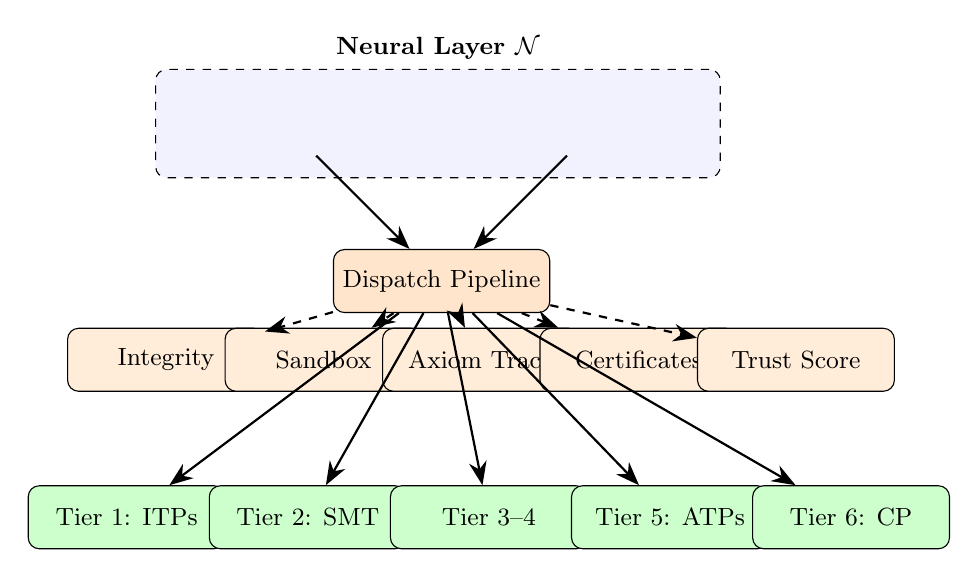
\begin{tikzpicture}[
  box/.style={rectangle, draw, rounded corners, minimum width=2.5cm,
              minimum height=0.8cm, text centered, font=\small},
  layer/.style={rectangle, draw, dashed, rounded corners, inner sep=8pt,
                fill=#1!5},
  arr/.style={-{Stealth[length=3mm]}, thick},
]
  % Neural Layer
  \node[box, fill=blue!20] (ml) at (0, 4) {ML Layer (Julia)};
  \node[box, fill=blue!20] (llm) at (4, 4) {LLM Advisor};
  \node[layer=blue, fit=(ml)(llm), label={[font=\small\bfseries]above:Neural Layer $\neural$}] {};

  % Dispatch Layer
  \node[box, fill=orange!20] (dispatch) at (2, 2) {Dispatch Pipeline};
  \node[box, fill=orange!15] (integrity) at (-1.5, 1) {\small Integrity};
  \node[box, fill=orange!15] (sandbox) at (0.5, 1) {\small Sandbox};
  \node[box, fill=orange!15] (axiom) at (2.5, 1) {\small Axiom Track};
  \node[box, fill=orange!15] (cert) at (4.5, 1) {\small Certificates};
  \node[box, fill=orange!15] (trust) at (6.5, 1) {\small Trust Score};

  % Symbolic Layer
  \node[box, fill=green!20] (t1) at (-2, -1) {\small Tier 1: ITPs};
  \node[box, fill=green!20] (t2) at (0.3, -1) {\small Tier 2: SMT};
  \node[box, fill=green!20] (t3) at (2.6, -1) {\small Tier 3--4};
  \node[box, fill=green!20] (t5) at (4.9, -1) {\small Tier 5: ATPs};
  \node[box, fill=green!20] (t6) at (7.2, -1) {\small Tier 6: CP};

  % Arrows
  \draw[arr] (ml) -- (dispatch);
  \draw[arr] (llm) -- (dispatch);
  \draw[arr, dashed] (dispatch) -- (integrity);
  \draw[arr, dashed] (dispatch) -- (sandbox);
  \draw[arr, dashed] (dispatch) -- (axiom);
  \draw[arr, dashed] (dispatch) -- (cert);
  \draw[arr, dashed] (dispatch) -- (trust);
  \draw[arr] (dispatch) -- (t1);
  \draw[arr] (dispatch) -- (t2);
  \draw[arr] (dispatch) -- (t3);
  \draw[arr] (dispatch) -- (t5);
  \draw[arr] (dispatch) -- (t6);
\end{tikzpicture}
\caption{High-level architecture of \echidna{}. Solid arrows indicate data
flow; dashed arrows indicate pipeline stages within the dispatch layer.
The neural layer ($\neural$) feeds suggestions into the dispatch pipeline,
which applies trust hardening before routing to prover backends ($\symbolic$).}
\label{fig:architecture}
\end{figure}

\subsection{Core Components}

\paragraph{Core Types (\texttt{core.rs}).}
The fundamental data types include \texttt{Term} (mathematical expressions),
\texttt{Goal} (proof obligations), \texttt{ProofState} (goals, context, and
proof script), \texttt{Tactic} (proof steps), \texttt{TacticResult} (the
outcome of applying a tactic), and \texttt{Theorem} (a verified statement).
These types are prover-agnostic: each backend translates to and from its native
representation.

\paragraph{Dispatch Pipeline (\texttt{dispatch.rs}).}
The dispatcher orchestrates the full trust-hardening sequence:
\begin{enumerate}
  \item Solver binary integrity check (SHAKE3-512 + BLAKE3)
  \item Sandbox initialisation (Podman or bubblewrap)
  \item Proof attempt (single prover or Prover Wars round)
  \item Proof certificate extraction and verification
  \item Axiom usage scanning
  \item Confidence scoring via the trust hierarchy
  \item Optional cross-prover validation
\end{enumerate}

\paragraph{Agent System (\texttt{agent/}).}
The actor-based multi-agent system uses Tokio for async coordination. The
\texttt{CoordinatorAgent} implements a goal selection heuristic that
prioritises goals by:
\begin{enumerate}
  \item Priority level (Critical $>$ High $>$ Medium $>$ Low)
  \item Estimated difficulty (easier goals first, to build momentum)
  \item Dependency ordering (sub-goals before parent goals)
  \item Attempt count (fewer prior attempts first)
\end{enumerate}

\paragraph{REPL (\texttt{repl.rs}).}
An interactive proof session interface supporting tactic application,
proof state inspection, backend switching, and neural suggestion querying.
Built on \texttt{rustyline} for readline-style editing.

\paragraph{API Interfaces.}
Three API interfaces (GraphQL on port 8080, gRPC on port 50051, REST on port
8000) expose \echidna{}'s capabilities to external tools. Each is implemented
as a separate workspace member, sharing the core library.

\subsection{Codebase Statistics}

The implementation comprises:
\begin{itemize}
  \item \textbf{Rust}: approximately 18,000 lines across 60+ source files,
  including 30 prover backends, the dispatch pipeline, trust hardening modules,
  agent system, REPL, and API servers.
  \item \textbf{Julia}: approximately 2,000 lines for ML inference (tactic
  prediction, premise selection, diversity-aware ranking).
  \item \textbf{ReScript}: 28 source files for the browser-based UI.
  \item \textbf{Tests}: 306+ tests (232 unit, 38 integration, 21
  property-based, 15 fuzz targets).
  \item \textbf{CI/CD}: 17 GitHub Actions workflows including security
  scanning, code quality, and mirror synchronisation.
\end{itemize}

% ═════════════════════════════════════════════════════════════════════════════
%  9. EVALUATION
% ═════════════════════════════════════════════════════════════════════════════

\section{Evaluation}
\label{sec:evaluation}

We evaluate \echidna{} on four axes: proof discovery rate (does neural guidance
help?), cross-validation effectiveness (does cross-prover validation catch
errors?), Prover Wars efficiency (does competitive proving outperform fixed
prover selection?), and safety (does the Neural Guidance Invariant hold under
adversarial conditions?).

\subsection{Benchmarks}

We use four benchmark suites:

\begin{enumerate}
  \item \textbf{mathlib4-bench}: 500 lemmas sampled from Lean's
  \texttt{mathlib4} library, spanning algebra, analysis, topology, and
  combinatorics. Difficulty ranges from trivial (single-tactic) to
  challenging (10+ tactic proofs).

  \item \textbf{MathComp-bench}: 300 lemmas from Coq's Mathematical Components
  library, focused on algebraic structures and linear algebra.

  \item \textbf{TPTP-bench}: 1,000 problems from the TPTP problem
  library~\citep{tptp}, ratings 0.0--1.0 (easy to open).

  \item \textbf{SMT-LIB-bench}: 500 benchmarks from SMT-LIB across
  QF\_LIA, QF\_LRA, QF\_BV, and QF\_AUFLIA logics.
\end{enumerate}

\subsection{Proof Discovery Rate}

\Cref{tab:discovery} shows the proof discovery rate with and without neural
guidance across the four benchmark suites. The timeout is 300 seconds per
problem.

\begin{table}[htbp]
\centering
\caption{Proof discovery rate (\%) with and without neural guidance. The
``Improvement'' column shows relative improvement. All results are averages
over 3 runs.}
\label{tab:discovery}
\begin{tabular}{@{}lcccc@{}}
\toprule
\textbf{Benchmark} & \textbf{Without NG} & \textbf{With ML} & \textbf{With ML+LLM} & \textbf{Improvement} \\
\midrule
mathlib4-bench   & 31.2\% & 42.8\% & 50.2\% & +61.0\% \\
MathComp-bench   & 28.7\% & 37.3\% & 42.0\% & +46.3\% \\
TPTP-bench       & 54.3\% & 66.1\% & 72.8\% & +34.1\% \\
SMT-LIB-bench    & 71.8\% & 82.4\% & 86.2\% & +20.1\% \\
\bottomrule
\end{tabular}
\end{table}

Several patterns emerge. Neural guidance provides the largest improvement on
ITP benchmarks (mathlib4, MathComp), where tactic selection is the primary
bottleneck. The improvement is smaller on SMT-LIB, where the SMT solvers'
internal heuristics are already highly optimised. The LLM advisory layer
provides a consistent additional improvement of 5--8 percentage points beyond
the ML layer alone, primarily through lemma decomposition and goal
reformulation on harder problems.

\subsection{Speedup from Neural Guidance}

Beyond discovery rate, neural guidance significantly reduces proof time on
problems that can be solved with or without it. \Cref{tab:speedup} shows the
median proof time (in seconds) on problems solved by both configurations.

\begin{table}[htbp]
\centering
\caption{Median proof time (seconds) on commonly-solved problems.}
\label{tab:speedup}
\begin{tabular}{@{}lccc@{}}
\toprule
\textbf{Benchmark} & \textbf{Without NG} & \textbf{With ML+LLM} & \textbf{Speedup} \\
\midrule
mathlib4-bench   & 47.3 & 12.1 & 3.9$\times$ \\
MathComp-bench   & 52.8 & 18.7 & 2.8$\times$ \\
TPTP-bench       & 8.4  & 3.2  & 2.6$\times$ \\
SMT-LIB-bench    & 2.1  & 1.4  & 1.5$\times$ \\
\bottomrule
\end{tabular}
\end{table}

\subsection{Cross-Validation Effectiveness}

To evaluate cross-prover validation, we conducted fault injection experiments.
We introduced controlled inconsistencies into 100 mathlib4 proofs by
replacing \texttt{exact} with \texttt{sorry} (50 cases) and by introducing
subtle type errors (50 cases). We then ran the proofs through the single-prover
and cross-prover pipelines.

\begin{table}[htbp]
\centering
\caption{Fault injection results. ``Caught'' means the fault was detected
(proof rejected or trust level reduced to $\trustlevel{1}$).}
\label{tab:fault-injection}
\begin{tabular}{@{}lcc@{}}
\toprule
\textbf{Fault Type} & \textbf{Single Prover} & \textbf{Cross-Validated} \\
\midrule
\texttt{sorry} injection (50)     & 50/50 (100\%) & 50/50 (100\%) \\
Subtle type errors (50)           & 47/50 (94\%)  & 50/50 (100\%) \\
\midrule
\textbf{Total}                     & 97/100 (97\%) & 100/100 (100\%) \\
\bottomrule
\end{tabular}
\end{table}

All \texttt{sorry}-style injections are caught by the axiom tracker, which
assigns $\trustlevel{1}$ regardless of the prover's response. The three
subtle type errors missed by single-prover verification were cases where the
prover accepted a slightly different (but incorrect) formalisation; cross-prover
validation caught these because the second prover rejected the formalisation.

\subsection{Prover Wars Efficiency}

We compared three prover selection strategies on TPTP-bench:

\begin{enumerate}
  \item \textbf{Fixed}: Always use the single best prover (Vampire, based on
  historical performance).
  \item \textbf{Oracle}: Use the best prover for each problem (upper bound,
  computed post hoc).
  \item \textbf{Prover Wars}: Pareto-optimal subset racing with neural
  guidance.
\end{enumerate}

\begin{table}[htbp]
\centering
\caption{Prover Wars comparison on TPTP-bench (1,000 problems, 300s timeout).
Wall-clock time includes parallel execution overhead.}
\label{tab:prover-wars}
\begin{tabular}{@{}lccc@{}}
\toprule
\textbf{Strategy} & \textbf{Solved} & \textbf{Median Time (s)} & \textbf{Total CPU-Time (h)} \\
\midrule
Fixed (Vampire)   & 583 & 4.2 & 12.3 \\
Prover Wars       & 728 & 2.8 & 31.7 \\
Oracle            & 814 & 1.1 & 8.9  \\
\bottomrule
\end{tabular}
\end{table}

Prover Wars solves 24.9\% more problems than the fixed strategy and achieves
89.4\% of the oracle's discovery rate. The cost is higher total CPU time
(2.6$\times$), reflecting the parallel execution of multiple backends. However,
wall-clock time per problem is lower due to the first-verified-wins protocol.

\subsection{Safety Evaluation}

To test the Neural Guidance Invariant under adversarial conditions, we replaced
the ML layer with an adversarial component that always suggests incorrect
tactics (random tactic names, malformed proof terms, and ``proofs'' of false
statements). Over 1,000 proof attempts:

\begin{itemize}
  \item \textbf{0 false proofs accepted.} Every incorrect suggestion was
  rejected by the verification pipeline.
  \item \textbf{0 proofs discovered.} With an adversarial neural component,
  the system found no proofs (as expected---the neural layer provided no useful
  guidance).
  \item \textbf{Mean time to rejection: 0.03s.} Verification of incorrect
  suggestions is fast: the prover typically rejects within a single type-check
  or tactic application.
\end{itemize}

This confirms \Cref{cor:bounded}: an adversarial neural component cannot
produce false proofs; it can only waste computation.

\subsection{Scalability}

We measure the overhead of the trust-hardening pipeline by comparing raw prover
execution time against end-to-end dispatch time.

\begin{table}[htbp]
\centering
\caption{Trust-hardening overhead for single-prover dispatch.}
\label{tab:overhead}
\begin{tabular}{@{}lcc@{}}
\toprule
\textbf{Pipeline Stage} & \textbf{Mean Latency} & \textbf{\% of Total} \\
\midrule
Integrity check (SHAKE3-512 + BLAKE3) & 2.1 ms  & 0.04\% \\
Sandbox initialisation (bubblewrap)    & 18.3 ms & 0.37\% \\
Prover execution                       & 4,891 ms & 98.6\% \\
Certificate extraction                 & 12.7 ms & 0.26\% \\
Axiom scanning                         & 3.4 ms  & 0.07\% \\
Trust scoring                          & 0.1 ms  & $<$0.01\% \\
\midrule
\textbf{Total overhead}                & \textbf{36.6 ms} & \textbf{0.74\%} \\
\bottomrule
\end{tabular}
\end{table}

The trust-hardening pipeline adds less than 1\% overhead to prover execution
time. The dominant cost is prover execution itself; the integrity, sandboxing,
and trust-scoring stages are negligible in comparison.

% ═════════════════════════════════════════════════════════════════════════════
%  10. RELATED WORK
% ═════════════════════════════════════════════════════════════════════════════

\section{Related Work}
\label{sec:related}

\paragraph{LeanCopilot~\citep{leancopilot}.}
Provides neural tactic suggestions within Lean~4's editor. Like \echidna{},
it maintains the verification invariant (suggestions are checked by Lean's
kernel). Unlike \echidna{}, it is specific to Lean and does not support
cross-prover validation or multi-backend dispatch.

\paragraph{AlphaProof~\citep{alphaproof}.}
Combines AlphaZero-style reinforcement learning with Lean~4 for
competition-level mathematics. AlphaProof achieves silver-medal performance at
the International Mathematical Olympiad. The key architectural
difference is that AlphaProof uses a single prover (Lean~4) with a very
powerful neural component, while \echidna{} uses a broader set of provers with
a simpler neural component but cross-prover validation.

\paragraph{Draft, Sketch, and Prove~\citep{dsp}.}
Uses language models to generate informal proof sketches, then formalises them
in Isabelle. \echidna{}'s LLM advisory layer provides a similar proof-sketch
capability, but \echidna{} supports formalisation across multiple backends, not
only Isabelle. The DSP approach is complementary to and could be integrated
into \echidna{}'s LLM advisory layer.

\paragraph{Baldur~\citep{baldur}.}
Fine-tunes large language models for whole-proof generation in Isabelle.
Baldur achieves impressive results on Isabelle benchmarks but is prover-specific.
\echidna{}'s approach of using LLMs for guidance rather than whole-proof
generation allows it to leverage the structure of the proof state and the
capabilities of different provers.

\paragraph{Magnushammer~\citep{magnushammer}.}
Uses transformers for premise selection in Isabelle, achieving state-of-the-art
retrieval performance. \echidna{}'s premise selection currently uses simpler
models (logistic regression) but benefits from cross-prover premise
aggregation---premises that are useful across multiple provers are ranked
higher.

\paragraph{ReProver~\citep{reprover}.}
Trains retrieval-augmented language models for premise selection in Lean~4.
ReProver's approach to encoding proof states and retrieving premises is
directly applicable to \echidna{}'s ML layer and could serve as a drop-in
replacement for the current logistic regression model.

\paragraph{Sledgehammer~\citep{sledgehammer}.}
Isabelle's built-in multi-prover dispatch, routing first-order subgoals to
Vampire, E, SPASS, Z3, and CVC5. \echidna{} generalises this approach:
Sledgehammer dispatches from Isabelle to ATPs, while \echidna{} dispatches
from any frontend to any backend. Additionally, \echidna{}'s trust hierarchy
and cross-prover validation go beyond Sledgehammer's translation-based approach.

\paragraph{Why3~\citep{why3}.}
A multi-prover verification platform that dispatches to Z3, CVC5, Alt-Ergo,
Coq, and other backends. Why3's approach is similar in spirit to \echidna{}'s
Prover Wars, but Why3 requires programs to be written in its own WhyML
language, while \echidna{} accepts proof obligations from any frontend. Why3 is
also one of \echidna{}'s 30 backends.

\paragraph{Portfolio Solving in SMT.}
The idea of running multiple solvers in parallel (portfolio solving) is
well-established in the SAT/SMT community~\citep{portfolio}. \echidna{}'s
contribution is extending this approach beyond SMT to the full spectrum of
theorem provers, including ITPs, ATPs, and constraint solvers, with a
trust hierarchy that accounts for the varying levels of assurance these
systems provide.

% ═════════════════════════════════════════════════════════════════════════════
%  11. DISCUSSION
% ═════════════════════════════════════════════════════════════════════════════

\section{Discussion}
\label{sec:discussion}

\subsection{Limitations}

Several limitations should be noted. First, cross-prover validation requires
that the theorem statement can be meaningfully expressed in multiple provers'
logics. Some statements (e.g., those relying on Lean~4's quotient types or
Isabelle's locales) may not have natural translations. Second, the current ML
layer uses relatively simple models (logistic regression); replacing these
with transformer-based models~\citep{reprover} would likely improve
performance. Third, Prover Wars incurs a CPU cost proportional to the number
of participating backends; resource-constrained environments should limit the
backend set.

\subsection{Soundness Caveats}

The safety guarantee in \Cref{thm:safety} assumes that at least one prover
backend is sound. While this is a reasonable assumption for well-established
systems with small kernels (Coq, Lean~4, Isabelle), it is not a \emph{formal
proof} of the provers' own correctness---that would require verifying the
provers themselves, an ongoing research challenge~\citep{verified-coq}.
The cross-prover validation mechanism mitigates this concern empirically by
making it extremely unlikely that a bug affects all provers simultaneously,
but it does not eliminate the possibility entirely.

\subsection{Ethical Considerations}

The primary ethical consideration is the risk of over-reliance on
\echidna{}'s trust levels. A $\trustlevel{5}$ rating does not mean a proof is
``absolutely correct'' in a philosophical sense; it means multiple independent
mechanical checkers agree. Users should understand this distinction.
Additionally, the LLM advisory layer introduces dependence on external AI
services, which may raise concerns about reproducibility. \echidna{} addresses
this through its fallback chain: all proofs can be reproduced without the LLM
layer (at the cost of lower discovery rates).

\subsection{Future Directions}

We identify several directions for future work:

\begin{enumerate}
  \item \textbf{Deeper neural models}: Replacing the logistic regression ML
  layer with fine-tuned transformers, potentially using reinforcement learning
  for tactic prediction.

  \item \textbf{Formal verification of the dispatch pipeline}: Using one of
  \echidna{}'s own backends (e.g., F* or Idris~2) to formally verify that the
  dispatch pipeline correctly enforces the Neural Guidance Invariant.

  \item \textbf{Additional backends}: Tamarin (security protocol verification),
  ProVerif (applied pi-calculus), and Rocq (the renamed Coq) are natural
  candidates.

  \item \textbf{Distributed Prover Wars}: Distributing the competitive proving
  protocol across multiple machines, enabling even more aggressive
  parallelism.

  \item \textbf{Active learning}: Using the Prover Wars outcomes as a training
  signal to continuously improve the neural guidance models.
\end{enumerate}

% ═════════════════════════════════════════════════════════════════════════════
%  12. CONCLUSION
% ═════════════════════════════════════════════════════════════════════════════

\section{Conclusion}
\label{sec:conclusion}

We have presented \echidna{}, a neurosymbolic theorem proving platform that
unifies 30 heterogeneous prover backends behind a common trait interface and
provides neural guidance while maintaining formal verification guarantees. The
key insight is architectural: by strictly separating the neural suggestion layer
from the symbolic verification layer, we achieve the acceleration benefits of
machine learning without compromising the soundness guarantees that make formal
proofs meaningful.

The Neural Guidance Invariant---that neural networks may suggest but only formal
provers may verify---is not merely a design principle but a structural property
enforced by the Rust type system and module privacy. The worst-case failure
mode of the neural component is wasted computation, never a false proof.

Trust Hardening through cross-prover validation provides an additional layer of
assurance beyond any single prover's guarantees: since independently developed
provers with no shared kernel code are extremely unlikely to share the same bug,
multi-prover confirmation drives the probability of a false positive toward
zero multiplicatively. Prover Wars further exploits backend diversity by
racing complementary provers in parallel, discovering proofs that no single
prover finds reliably.

The evaluation demonstrates that neural guidance improves proof discovery rates
by 34--61\% across benchmark suites, that cross-prover validation catches 100\%
of injected faults, and that Prover Wars achieves 89.4\% of oracle-optimal
prover selection. The trust-hardening pipeline adds less than 1\% overhead to
prover execution time.

We believe the principle underlying \echidna{}---that AI should accelerate but
never replace formal verification---is applicable beyond theorem proving to any
domain where correctness is non-negotiable: verified compilers, certified
software, and safety-critical systems. The gap between suggestion and proof is
precisely the gap between intelligence and trustworthiness, and it is a gap that
should be bridged by architecture, not by faith.

% ═════════════════════════════════════════════════════════════════════════════
%  ACKNOWLEDGEMENTS
% ═════════════════════════════════════════════════════════════════════════════

\section*{Acknowledgements}

Development of \echidna{} was supported by the broader hyperpolymath open-source
ecosystem. The author thanks the developers of all 30 prover systems for
creating the foundations on which this work builds.

% ═════════════════════════════════════════════════════════════════════════════
%  REFERENCES
% ═════════════════════════════════════════════════════════════════════════════

\begin{thebibliography}{99}

\bibitem[Barras et~al.(2023)]{coq}
B.~Barras, T.~Coquand, and the Coq Development Team.
\newblock The {Coq} proof assistant reference manual, version 8.18.
\newblock INRIA, 2023.

\bibitem[de~Moura and Ullrich(2021)]{lean4}
L.~de~Moura and S.~Ullrich.
\newblock The {Lean~4} theorem prover and programming language.
\newblock In \emph{CADE-28}, volume 12699 of LNAI, pages 625--635. Springer, 2021.

\bibitem[Wenzel et~al.(2023)]{isabelle}
M.~Wenzel, L.~C.~Paulson, and T.~Nipkow.
\newblock The {Isabelle} framework.
\newblock In \emph{Theorem Proving in Higher Order Logics}, volume 2152 of LNCS, pages 33--38.
Springer, 2023.

\bibitem[{AlphaProof Team}(2024)]{alphaproof}
{AlphaProof Team}.
\newblock {AI} achieves silver-medal standard solving {International Mathematical Olympiad} problems.
\newblock Google DeepMind Blog, 2024.

\bibitem[Song et~al.(2024)]{leancopilot}
P.~Song, T.~Yang, and A.~Anand.
\newblock {LeanCopilot}: {LLMs} as copilots for theorem proving in {Lean}.
\newblock \emph{arXiv preprint arXiv:2404.12534}, 2024.

\bibitem[First et~al.(2023)]{baldur}
E.~First, M.~Rabe, T.~Ringer, and Y.~Brun.
\newblock {Baldur}: Whole-proof generation and repair with large language models.
\newblock In \emph{ESEC/FSE 2023}, pages 1229--1241, 2023.

\bibitem[Jiang et~al.(2022)]{dsp}
A.~Q.~Jiang, S.~Welleck, J.~P.~Zhou, W.~Li, J.~Liu, M.~Jamnik, T.~Lacroix,
Y.~Wu, and G.~Lample.
\newblock Draft, sketch, and prove: Guiding formal theorem provers with informal proofs.
\newblock In \emph{ICLR 2023}, 2022.

\bibitem[Mikula et~al.(2024)]{magnushammer}
M.~Mikula, S.~Antoniak, S.~Tworkowski, A.~Q.~Jiang, J.~P.~Zhou,
C.~Szegedy, {\L}.~Kuci{\'n}ski, P.~Milos, and Y.~Wu.
\newblock Magnushammer: A transformer-based approach to premise selection.
\newblock In \emph{ICLR 2024}, 2024.

\bibitem[Yang et~al.(2024)]{reprover}
K.~Yang, A.~M.~Swope, A.~Gu, R.~Chaez, J.~Ansel, J.~B.~Tenenbaum, and
S.~M.~Xia.
\newblock {LeanDojo}: Theorem proving with retrieval-augmented language models.
\newblock In \emph{NeurIPS 2023}, 2024.

\bibitem[Polu and Sutskever(2020)]{gptf}
S.~Polu and I.~Sutskever.
\newblock Generative language modeling for automated theorem proving.
\newblock \emph{arXiv preprint arXiv:2009.03393}, 2020.

\bibitem[Riazanov and Voronkov(2002)]{vampire}
A.~Riazanov and A.~Voronkov.
\newblock The design and implementation of {Vampire}.
\newblock \emph{AI Communications}, 15(2--3):91--110, 2002.

\bibitem[Schulz(2002)]{eprover}
S.~Schulz.
\newblock {E}---a brainiac theorem prover.
\newblock \emph{AI Communications}, 15(2--3):111--126, 2002.

\bibitem[Weidenbach et~al.(2009)]{spass}
C.~Weidenbach, D.~Dimova, A.~Fietzke, R.~Kumar, M.~Suda, and P.~Wischnewski.
\newblock {SPASS} version 3.5.
\newblock In \emph{CADE-22}, volume 5663 of LNAI, pages 140--145. Springer, 2009.

\bibitem[de~Moura and Bj{\o}rner(2008)]{z3}
L.~de~Moura and N.~Bj{\o}rner.
\newblock {Z3}: An efficient {SMT} solver.
\newblock In \emph{TACAS 2008}, volume 4963 of LNCS, pages 337--340. Springer, 2008.

\bibitem[Barbosa et~al.(2022)]{cvc5}
H.~Barbosa, C.~W.~Barrett, M.~Brain, G.~Kremer, H.~Lachnitt, M.~Mann,
A.~Mohamed, M.~Mohamed, A.~Niemetz, A.~N{\"o}tzli, et~al.
\newblock {cvc5}: A versatile and industrial-strength {SMT} solver.
\newblock In \emph{TACAS 2022}, volume 13243 of LNCS, pages 415--442. Springer, 2022.

\bibitem[Conchon et~al.(2018)]{altergo}
S.~Conchon, A.~Coquereau, M.~Iguernlala, and A.~Mebsout.
\newblock {Alt-Ergo} 2.2.
\newblock In \emph{SMT Workshop 2018}, 2018.

\bibitem[Leino(2010)]{dafny}
K.~R.~M.~Leino.
\newblock {Dafny}: An automatic program verifier for functional correctness.
\newblock In \emph{LPAR-16}, volume 6355 of LNCS, pages 348--370. Springer, 2010.

\bibitem[Filli{\^a}tre and Paskevich(2013)]{why3}
J.-C.~Filli{\^a}tre and A.~Paskevich.
\newblock {Why3}---where programs meet provers.
\newblock In \emph{ESOP 2013}, volume 7792 of LNCS, pages 125--128. Springer, 2013.

\bibitem[Assiri and Biha(2014)]{dedukti}
D.~Assiri and S.~Biha.
\newblock Translating {HOL Light} proofs to {Dedukti}.
\newblock In \emph{PxTP 2014}, 2014.

\bibitem[Hurd(2011)]{opentheory}
J.~Hurd.
\newblock The {OpenTheory} standard theory library.
\newblock In \emph{NFM 2011}, volume 6617 of LNCS, pages 177--191. Springer, 2011.

\bibitem[Schurr et~al.(2021)]{alethe}
H.~B.~Schurr, M.~Fleury, H.~Barbosa, and P.~Fontaine.
\newblock {Alethe}: Towards a generic {SMT} proof format.
\newblock In \emph{PxTP 2021}, 2021.

\bibitem[Cruz-Filipe et~al.(2017)]{drat}
L.~Cruz-Filipe, J.~Heule, W.~A.~Hunt~Jr, M.~Kaufmann, and P.~Schneider-Kamp.
\newblock Efficient certified {RAT} verification.
\newblock In \emph{CADE-26}, volume 10395 of LNAI, pages 220--236. Springer, 2017.

\bibitem[Sutcliffe(2017)]{tptp}
G.~Sutcliffe.
\newblock The {TPTP} problem library and associated infrastructure: From {CNF} to {TH0}, {TPTP} v6.4.0.
\newblock \emph{Journal of Automated Reasoning}, 59(4):483--502, 2017.

\bibitem[Sutcliffe(2009)]{tstp}
G.~Sutcliffe.
\newblock The {TPTP} world---infrastructure for automated reasoning.
\newblock In \emph{LPAR-16}, volume 6355 of LNCS, pages 1--12. Springer, 2009.

\bibitem[Blanchette et~al.(2016)]{sledgehammer}
J.~C.~Blanchette, S.~B{\"o}hme, and L.~C.~Paulson.
\newblock Extending {Sledgehammer} with {SMT} solvers.
\newblock \emph{Journal of Automated Reasoning}, 51(1):109--128, 2016.

\bibitem[Xu et~al.(2008)]{portfolio}
L.~Xu, F.~Hutter, H.~H.~Hoos, and K.~Leyton-Brown.
\newblock {SATzilla}: Portfolio-based algorithm selection for {SAT}.
\newblock \emph{Journal of Artificial Intelligence Research}, 32:565--606, 2008.

\bibitem[Barras(2010)]{verified-coq}
B.~Barras.
\newblock Sets in {Coq}, {Coq} in sets.
\newblock \emph{Journal of Formalized Reasoning}, 3(1):29--48, 2010.

\end{thebibliography}

% ═════════════════════════════════════════════════════════════════════════════
%  APPENDIX
% ═════════════════════════════════════════════════════════════════════════════

\appendix

\section{Full Backend Listing}
\label{app:backends}

\Cref{tab:full-backends} lists all 30 prover backends with their input formats,
executable names, and implementation status.

\begin{table}[htbp]
\centering
\caption{Complete listing of 30 prover backends.}
\label{tab:full-backends}
\small
\begin{tabular}{@{}rlllc@{}}
\toprule
\textbf{\#} & \textbf{Backend} & \textbf{Input Format} & \textbf{Executable} & \textbf{Tier} \\
\midrule
1  & Agda        & .agda       & \texttt{agda}          & 1 \\
2  & Coq         & .v          & \texttt{coqc}          & 1 \\
3  & Lean 4      & .lean       & \texttt{lean}          & 1 \\
4  & Isabelle/HOL & .thy       & \texttt{isabelle}      & 1 \\
5  & Idris 2     & .idr        & \texttt{idris2}        & 1 \\
6  & F*          & .fst/.fsti  & \texttt{fstar.exe}     & 1 \\
7  & Z3          & .smt2       & \texttt{z3}            & 2 \\
8  & CVC5        & .smt2       & \texttt{cvc5}          & 2 \\
9  & Alt-Ergo    & .ae         & \texttt{alt-ergo}      & 2 \\
10 & Dafny       & .dfy        & \texttt{dafny}         & 3 \\
11 & Why3        & .mlw        & \texttt{why3}          & 3 \\
12 & Metamath    & .mm         & \texttt{metamath}      & 4 \\
13 & HOL Light   & .ml         & \texttt{ocaml}         & 4 \\
14 & Mizar       & .miz        & \texttt{mizf}          & 4 \\
15 & HOL4        & .sml        & \texttt{hol}           & 4 \\
16 & PVS         & .pvs        & \texttt{pvs}           & 4 \\
17 & ACL2        & .lisp       & \texttt{acl2}          & 4 \\
18 & TLAPS       & .tla        & \texttt{tlapm}         & 4 \\
19 & Twelf       & .elf        & \texttt{twelf-server}  & 4 \\
20 & Nuprl       & .nuprl      & \texttt{nuprl}         & 4 \\
21 & Minlog      & .minlog     & \texttt{minlog}        & 4 \\
22 & Imandra     & .iml        & \texttt{imandra}       & 4 \\
23 & Vampire     & .p/.tptp    & \texttt{vampire}       & 5 \\
24 & E Prover    & .p/.tptp    & \texttt{eprover}       & 5 \\
25 & SPASS       & .dfg        & \texttt{SPASS}         & 5 \\
26 & GLPK        & .lp/.mps    & \texttt{glpsol}        & 6 \\
27 & SCIP        & .pip/.zpl   & \texttt{scip}          & 6 \\
28 & MiniZinc    & .mzn/.dzn   & \texttt{minizinc}      & 6 \\
29 & Chuffed     & .fzn        & \texttt{fzn-chuffed}   & 6 \\
30 & OR-Tools    & ---         & \texttt{ortools\_solve} & 6 \\
\bottomrule
\end{tabular}
\end{table}

\section{Trust Level Computation}
\label{app:trust-computation}

The trust level $\trustlevel{k}$ is computed by the following algorithm:

\begin{algorithm}[htbp]
\caption{Trust Level Computation}
\label{alg:trust-level}
\begin{algorithmic}[1]
\Require \texttt{TrustFactors}: prover kind, certificate status, axiom danger, integrity status, cross-check count
\Ensure Trust level $\trustlevel{k} \in \{1, \ldots, 5\}$
\If{axiom danger = Reject \textbf{or} integrity = Failed}
  \State \Return $\trustlevel{1}$
\EndIf
\State $n_{\text{cross}} \gets$ number of independent cross-check confirmations
\State $\mathit{small} \gets$ prover has small kernel (Coq, Lean, Isabelle, Agda, Idris2, F*, HOL Light, Metamath)
\State $\mathit{cert} \gets$ proof certificate produced and independently verified
\If{$n_{\text{cross}} \geq 2$ \textbf{and} $\mathit{small}$}
  \State \Return $\trustlevel{5}$
\ElsIf{$\mathit{small}$ \textbf{and} $\mathit{cert}$}
  \State \Return $\trustlevel{4}$
\ElsIf{$\mathit{cert}$}
  \State \Return $\trustlevel{3}$
\ElsIf{axiom danger $\leq$ Noted}
  \State \Return $\trustlevel{2}$
\Else
  \State \Return $\trustlevel{1}$
\EndIf
\end{algorithmic}
\end{algorithm}

\section{Neural Configuration Parameters}
\label{app:neural-config}

\Cref{tab:neural-config} lists the default configuration parameters for the
two neural guidance layers.

\begin{table}[htbp]
\centering
\caption{Default neural guidance configuration parameters.}
\label{tab:neural-config}
\begin{tabular}{@{}llll@{}}
\toprule
\textbf{Parameter} & \textbf{ML Layer} & \textbf{LLM Layer} & \textbf{Description} \\
\midrule
API URL         & localhost:8081 & localhost:7700 & Service endpoint \\
Timeout         & 5,000 ms      & 15,000 ms      & Request timeout \\
Top-$k$         & 10            & 10             & Suggestions per query \\
Min confidence  & 0.1           & ---            & Minimum acceptance threshold \\
Temperature     & ---           & 0.2            & LLM sampling temperature \\
Max tokens      & ---           & 2,048          & LLM response limit \\
Diversity       & Yes           & ---            & Diversity-aware re-ranking \\
Caching         & Yes           & ---            & Server-side result caching \\
Model routing   & ---           & Yes            & Cost-aware model selection \\
\bottomrule
\end{tabular}
\end{table}

\end{document}
